\documentclass[12pt, letterpaper]{article}
\usepackage[serbian]{babel}
\usepackage{hyperref}
\usepackage{graphicx}

\title{AI koji generiše sliku na osnovu teksta}
\author{Budimir Nkola 178/2021\\Trajković Miljan 354/2022\\Cvejić Miloš 346/2021\\Bajić Bogdan 122/2021}

\begin{document}


\maketitle

\begin{tableofcontents}
\end{tableofcontents}

\pagebreak 

\section{Uvod} 

\subsection*{Veštačka inteligencija} 

Veštačka inteligencija, iliti AI (skraćeno od eng. artifitial intelligence) predstavlja podoblast računarstva koja omogućava računarima da realizuju funkcije koje su karakteristika ljudskog razmišljanja, odnosno da što vernije imitiraju rad ljudskog mozga. Veštačka inteligencija je počela da se razvija tokom druge polovine dvadesetog veka, a tokom proteklih godina taj razvoj je počeo da se sve više i više ubrzava. Veštačka inteligencija se, iako je još uvek tek u svojim početnim fazama, koristi u raznim oblastima za rešavanje mnogih problema. \cite{kljucJedan} 

  

Neka od čestih mesta na kojima se upotrebljava veštačka inteligencija su obrada podataka, prevođenje jezika, prepoznavanje slika, razvoj softvera, elektronska trgovina (e-commerce), video igre, medicina, napredni internet pretraživači, sistemi preporuke (poput onih koje koriste YouTube, Amazon, Netflix i slični), robotika, proizvodnja bespilotnih letelica i autonomnih automobila (poptut onih koje proizvodi Tesla), generisanje slika, kao i još mnogo drugih.  

  

Mašinsko učenje predstavlja podoblast veštačke inteligencije. Ono omogućava da računar “nauči” zadati šablon koji dobija kroz milione podataka i upotrebi ga kako bi mogao da oponaša taj isti tip ponašanja.   

  

Pristupi mašinskom učenju se generalno dele u tri različite kategorije (koje odgovaraju paradigmama učenja), u zavisnosti od prirode signala ili povratne informacije dostupne sistemu učenja. To su: učenje pod nadzorom (eng. supervised learning), polunadgledano učenje (eng. semi-supervised learning)), učenje bez nadzora (unsupervised learning) i učenje potkrepljenjem (reinforcement learning).  

  

Učenje pod nadzorom je paradigma mašinskog učenja kod koje postoji nadgledač koji predstavlja učitelja. Kod ovog tipa učenja, obučavamo računar koristeći podatke koji su ispravno označeni, nakon čega mu dajemo pristup novim podacima, koje on treba da analizira, prepozna i da zna šta treba da radi sa njima. Učenje bez nadzora je paradigma mašinskog učenja kod koje se računar obučava koristeći informacije koje nisu označene (za razliku od učenja pod nadzorom). Zadatak računara je da grupiše zadate podatke prema njihovim sličnostima, bez ikakve prethodne obuke. Učenje potkrepljenjem predstavlja paradigmu mašinskog učenja koja podseća na treniranje kućnog ljubimca. Radi se o nagrađivanju računara kada je radnja koju je učinio adekvatna. Na prvi pogled to podseća na učenje pod nadzorom, ali za razliku od tog tipa, kod učenja potkrepljenjem računar nema podatke koje koristi za buku, već uči iz sopstvenog iskustva. \cite{kljucDva} 

  

\subsection*{Šta je AI generator slika} 

AI generator slika predstavlja program koji generiše sliku na osnovu zahteva zadatog u obliku teksta koristeći veštačku inteligenciju. To funkcioniše tako što generator slika ima pristup bazi podataka u kojoj se nalazi veliki broj različitih slika, na osnovu kojih on uči da generiše nove slike. Kada generator slika dobije opis slike koju treba da generiše, on u bazi podataka proverava slike sa sličnim opisom i na osnovu njih generiše sliku koja podseća na njih.  

  

Slike generisane korišćenjem veštačke inteligencije često se koriste za pravljene reklama, postera, imitaciju poznatih dela, kao i za dobijanje inspiracije, ili prosto radi zabave.  

  

Neki od poznatih programa za generisanje slika na osnovu zadatog teksta su: 

\begin{itemize} 

\item[-] Jasper Art 

\item[-] Canva AI Art 

\item[-] Starry AI 

\item[-] Nightcafe 

\item[-] Dall-E 

\item[-] Pixray 

\item[-] Deep Dream Generator 

\item[-] Deep AI 

\item[-] ArtBreeder 

\item[-] Hypotenuse AI 

\item[-] Craiyon (DALL-E mini) 

\item[-] i drugi. 

\end{itemize} 

\cite{kljucTri} 

\pagebreak
\section{Kako funkcionišu AI generatori slika}
\subsection*{Preteče današnjih generatora}
Mnogi modeli veštačke inteligencije pa tako i generatori slika na osnovu teksta poput \textbf{DALL-E 2} i drugih, zasnovani su na prethodnim istraživanjima i prethodnim modelima iz ove oblasti.
Generisanje slika razvijalo se linearno i to prvobitno koriscenjem mreža koje koriste metode suparničkog učenja odnosno “Generative adversarial network” (GANs).

GANs su modeli mašinskog učenja obično sačinjeni od dve mreže, \textit{diskriminatora} i \textit{generatora}, koje međusobnim intereagovanjem treniraju jedna drugu. Naime, ako uzmemo na primer generisanje slika, zadatak diskriminatora je da što sigurnije i preciznije odredi da li je njemu zadata slika, prava fotografija iz neke baze podataka ili je to generisana slika. Sa druge strane, zadatak generatora je da prevari diskriminatora, odnosno da što bolje nauči šta sliku čini “pravom” i tako napravi sliku za koju se ne može utvrditi da li je ona prava ili ne. U tom slučaju interakcija ove dve mreže i njihovo treniranje se može posmatrati kao minimaks igra u kojoj se diskriminator trenira da maksimalno uveća verovatnoću tačnog određivanja klase slika, dok se generator trenira da maksimalno umanji verovatnoću da slike koje je generisao budu klasifikovane od strane diskriminatora kao generisane slike.\cite{gan1, gan2, ganvideo}

Ključna razlika između ovako opisanih mreža i najnovijih AI generatora slika je ta što se klasični GAN modeli obično razvijaju za neku konkretnu kategoriju fotografija(npr. popularni generator ljudskih lica)\cite{gen1} dok na drugoj strani generatori poput DALL-E 2, Stable Diffusion, Imagen-a su mnogo opštije namene i možemo im zadati tekstualni opis slike koju očekujemo od generatora. To zadavanje opisa se realizuje proširivanjem već pomenutih mreža tako što se generatoru prosleđuje uslov po kom će on generisati sliku.\cite{openai_dali, openai_glide, asembli} 
Formiranje ovog uslova je zapravo netrivijalna stvar jer najbolje realizacije generatora nisu one u kojima se kao uslov prosleđuje samo opis slike što je i pokazano u istraživanju \textbf{OpenAI} tima.\cite{openai_dali}

Arhitekture najnovijih generatora zasnovane su na jednoj od novijih tehnika nazvanoj difuzija(eng. diffusion) koja je inspirisana oblašću iz fizike - neravnotežna termodinamika. Naime, ako sipamo kap farbe u vodu, zakoni fizike nalažu da će ta kap da \textit{difunduje}\footnote{Difundovanje - proces spontanog raspršivanja materije i energije, prelazak iz zone više u zonu niže energije ili koncentracije} sve dok ne dođe u ravnotežu. Ovaj proces u prirodi je ireverzibilan. U mašinskom učenju, modeli difuzije nastoje da reše upravo ovaj problem, odnosno da nađu način kojim mogu doći do početne kapi farbe.\cite{asembli}

\subsection{Pregled arhitekture DALL-E 2 softvera}

Na primeru konkretnog generatora DALL-E 2 možemo videti prethodno opisane mreže i koju ulogu one imaju u jednom od najpoznatijih softvera za generisanje slika.

Za pocetak posmatraćemo takozvanu CLIP mrežu (skraćeno od Contrastive Language–Image Pre-training), koja je izuzetno bitna za treniranje osnovnih komponenti ovog generatora. Njen osnovni zadatak je da zadatu sliku poveže sa odgovarajućim unetim opisom. Primetimo da se na neki način generisanje slika može smatrati suprotnim procesom od pomenutog, a razlog zašto je ova mreža od ključnog značaja prilikom generisanja ćemo videti u nastavku teksta. Na ulazu CLIP mreže nalaze se dva kodera koji kodiraju zadatu sliku i njen opis u odgovarajući \textit{imbeding}\footnote{imbeding (eng. embedding) - rezultat preslikavanja skupa informacija u računarski zapis, vektor}, zasebice. Prilikom treniranja, CLIP nastoji da pomenute kodere nauči da imbeding slike i imbeding njenog opisa budu što sličniji jedan drugom.\cite{clip, openai_dali}

\begin{figure}[htp]
\centering
\includegraphics[width=0.6\textwidth]{clip.png}
\caption{Slika preuzeta sa OpenAI blog stranice}
\label{fig: clipslika}
\end{figure}

\pagebreak

Sama arhitektura Dall-E 2 softvera se sastoji iz dva dela: Prvi deo čini mreža prior\footnote{prior - označava ono što je pre nečega po redu ili hronološki.} koji na ulazu prima tekst imbeding (formiran CLIP kodiranjem tekstualnog opisa željene slike) koji preslikava u imbeding slike koji prosleđuje drugom delu ovog generatora - dekoderu. Sada dolazimo do ključnog značaja CLIP mreže. OpenAI tim se zapitao, da li je prior u ovom pristupu uopšte potreban. Iz tog razloga pokušali su da dekoderu proslede samo tekstualni opis, zatim tekstualni opis i tekst imbeding, a na kraju i imbeding slike dobijen pomoću prior-a. Iz tog eksperimenta su zaključili da slike generisane imbedingom slike daju značajno bolje rezulate u odnosu na druga dva slučaja.\cite{openai_dali}

Dekoder je generativni model realizovan pomenutom tehnikom difuzuje. Naime, slike se generišu iz nasumične količine \textit{Gausovog šuma}\footnote{Gausov šum (engl. Gaussian noise) - šum raspoređen korišćenjem Gausove normalne raspodele}. Zadatak generatornog dela je da pretpostavi koliko šuma je na slici i otkloni ga. Ovo je vrlo težak problem koji se uspešno rešava upravo difuzno i to na sledeći način: Otklanjanje šuma vrši se iterativno\cite{gen1}. U svakoj iteraciji pretpostavlja se koliko šuma je na slici koji se otklanja, a zatim se na dobijenu sliku dodaje skoro malo manja količina Gausovog šuma od prethodnog i prelazi u sledeću iteraciju. Kako bi dekoder znao šta uopšte treba da generiše, odnosno “šta se nalazi ispod šuma” prosleđuje mu se uslov. Kod ranijih projekata kao što su GLIDE i DALL-E\cite{openai_glide, openai_dali}, dekoderu se kao uslov direktno prosleđivao tekstualni opis željene slike. Dok se kod ovog modela zahvaljujući CLIP i prior mreži generatoru dodatno prosleđuju CLIP imbeding slike i teksta. Generisanje različitih slika i variranje u odnosu na jednu generisanu sliku se postiže tako što se dobijena slika propušta kroz CLIP koder kako bi se dobio njen imbeding slike, a onda se proces generisanja ponavlja sa novonastalim imbedingom. Na ovaj način dobija se slika koja ima iste elemente i stil prethodne slike, a različit raspored i neke trivijalne detalje koji se gube CLIP kodiranjem. Izlaz opisanog dela dekodera je slika formata 64x64.

Zato se na samom kraju ovog generatora slika rezolucije 64x64 prolazi kroz jos dva ekspanzivna koraka kojim se slika dovodi na rezoluciju 1024x1024. Ovi koraci su takođe realizovani difuznim tehnikama što doprinosi tome da slika na izlazu ima više detalja i bude maksimalno fotorealistična.\cite{openai_dali}

\begin{figure}[htp]
\centering
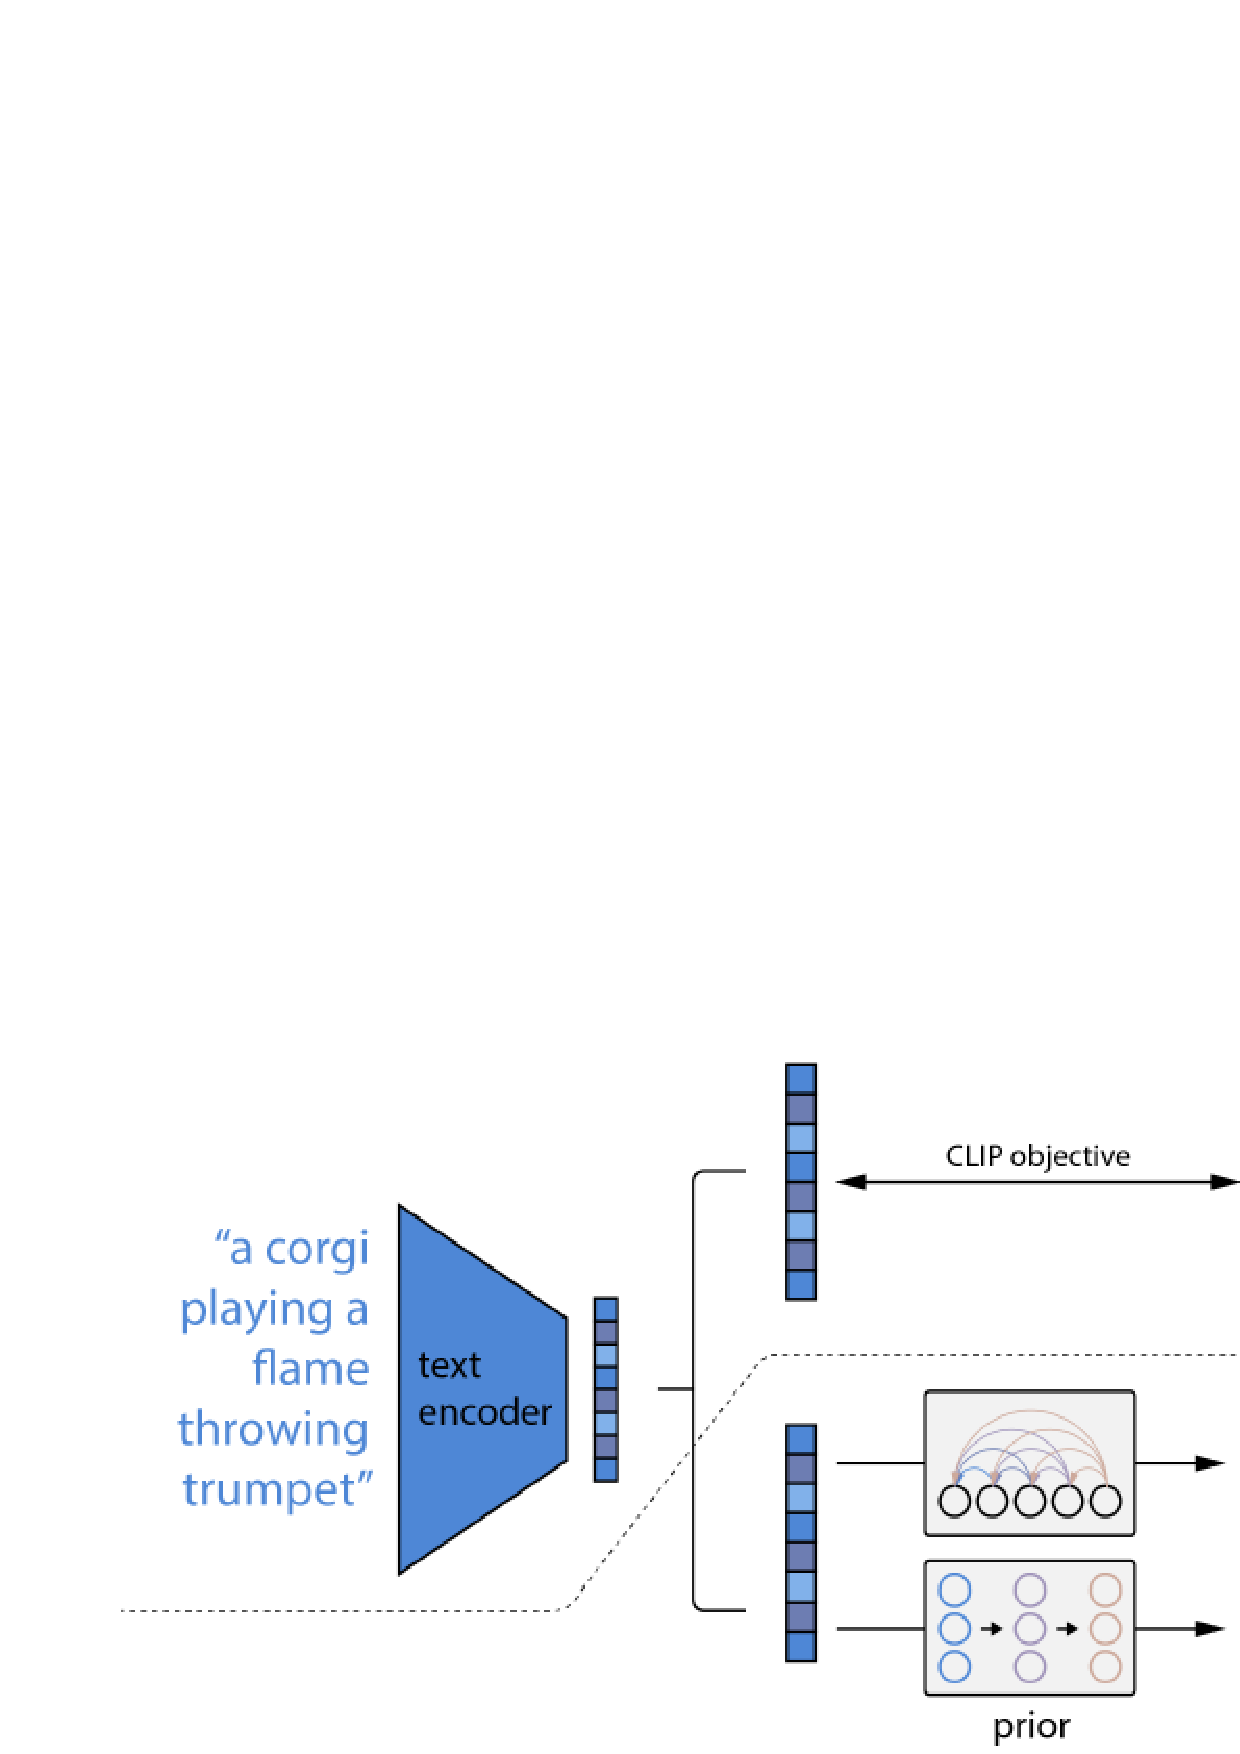
\includegraphics[width=1\textwidth]{dalle2.png}
\caption{Prikaz DALL-E 2 modela iz ptičije perspektive}
\label{fig: dalle2slika}
\end{figure}

\pagebreak

\section{Treniranje AI generatora slika}

Kako smo već objasnili neke od modela mašinskog učenja koji se koriste u generatorima slika može samo dodati neke ključne detalje koji su bitni kod ovako velikih projekata.

Za Trening softvera kao što je generator slika neophodne su ogromne baze podataka slika koje su pažljivo birane za ovaj trening. Naravno, kreiranje ovakvih baza podataka i prikupljanje slika generalno zahteva veliki broj ljudi koji rade na ovom projektu. Jedna od najzahtevnijih baza jeste The ImageNet baza slika na kojoj je radilo preko 25 hiljada ljudi koji su skupili 14 miliona slika na kojima se može naći dvadeset dve hiljade različitih objekata. Interesantno je to da OpenAI tim nije utrošio ovakve napore prilikom treniranja Dall-E 2 generatora. \cite{clip}

Već smo pričali o CLIP mreži. Tokom njenog treniranja ona prima parove slika i njihovih opisa. Te parove mreža pronalazi na internetu. Možemo primetiti da slike dobijene Gugl pretragom, kao i slike na društvenim mrežama poput Instagrama i Tvitera gotovo uvek imaju opise i lako im se pristupa. Samim tim trošak na građenje iscrpnih baza slika potpuno je prevaziđen.\cite{clip, openai_dali}

Treniranje dekodera svodi se na treniranje difuznog modela. Najbitnije je pomenuti jednu difuznu tehniku zvanu navođenje bez klasifikatora(eng. Classifier-free guidance). Ova tehnika podrazumeva da se generatoru u određenom broju slučaja prosleđeni CLIP imbeding postavljaju na nulu, čime je generator forsiran da napravi sliku samo na osnovu teksta. A tokom treniranja 50\% posto generacija izvršava se bez teksta, odnosno samo pomoću CLIP imbedinga.

Takođe, tokom treniranja mreža koje sliku rezolucije 64x64 proširuju na sliku rezolucije 1024x1024, slike koje dolaze na ulaz mogu biti malo zamućene korišćenjem Gausove normalne raspodele. Kao što smo rekli baš zbog ovih difuznih tehnika na izlazu dekodera dobijamo sliku rezolucije 1024x1024 koja je fotorealistična i može sadržati puno detalja.\cite{openai_dali}

\pagebreak

\section{Kako bilo ko može da koristi AI za generisanje slika}
Veštačka inteligencija koja generiše slike bila je jedna od gorućih tema u vestima ove godine zbog izuzetno brzog napretka ali i etičkih problema. Međutim, zašto bi, i kako, mogli da koristimo ove novotarije?

Motivacija za korišćenje:
\begin{itemize}
  \item[-] Može da generiše realistične, ili čak, hiperrealistične slike što se može koristiti u svrhu razvoja moderne umetnosti (npr. u filmovima za stvaranje zanimljivijih i privlačnijih scena natprirodnih pojava).
  \item[-] AI “razmišlja” van okvira što mu dozvoljava da generiše neke nikada pre viđene stvari koje mogu biti značajna inspiracija za nove ideje i projekte, kao i potencijalno otvaranje potpuno novih pravaca u umetnosti.
  \item[-] AI takođe konstanto evoluira i stvara nove i naprednije podatke, koje koristi da bi se unapređivao dalje. Tehnički, ovo mu omogućava da stalno proizvodi nove ideje, bez zasićenja, dakle izbegava “autorsku blokadu”.
\end{itemize}

Neki od izazova:
\begin{itemize}
    \item[-] Iako bi veštački genersiane slike mogle da zavaraju bilo kog čoveka, ipak će njima faliti ljudski dodir odnosno emocija kao i priča koja stoji iza stvaranja tog dela.
    \item[-] Čovek nema nikakvu kontrolu nad kreativnim procesom što znači da će AI stvarati isključivo na osnovu podataka pomoću kojih je istreniran, što takođe može dovesti do ponavljanja istih stvari u različitom svetlu, ili stvaranja besmislenih i dosadnih slika.
    \item[-] Etički problemi su svakako neizostavna stavka svake konverzacije o veštačkoj inteligenciji. Pitanja koja ovde postavljamo tiču se autorskih prava, prodavanja veštački generisanih slika i njihova zloupotreba. 
\end{itemize}

\subsection{DALL-E 2}
\textbf{DALL-E 2} kompanije OpenAI jedno je od glavnih imena u ovom prostoru. Čitav proces je zapravo prilično jednostavan – unesemo opis željene stvari i dobijemo sliku toga. Ali, ima još par stavki koje treba da držimo na umu da bi postigli savršen rezultat. 

Prvo, prijavimo se na zvanični sajt. Korišćenje AI-a nije u potpunosti besplatno. Po otvaranju naloga dobijate 50 “kredita” i svakog meseca po 15, s tim što se taj kredit ne prenosi, dok se kupljeni kredit prenosi (npr. možete kupiti 115 kredita za 15 dolara). Jedan kredit vam daje i jednu veštački generisanu sliku. Dužina samog opisa tj. \textit{prompt-a}\footnote{eng. to prompt - navesti} je 400 karaktera, a sam prompt može da primi \textit{sadržaj} i textit{modifikatore}. Sadržaj je npr. \textit{"usamljeni astrounaut na Marsu"}, a modifikator \textit{"misteriozno, sa puno boja, hiperrealistično"} (naravno, podrazumeva se da se reči unose na engleskom). Postoje i posebne knjige\cite{Prompt}, kao i eksperti, koji vam mogu pomoći kako da unesete savršeni prompt. Jedan od načina da postavite atmosferu jeste da koristite reči koje predstavljaju emocije ili vremensko razdoblje. Takođe možete i da unesete konkretni objektiv za kameru ili naziv pametnog telefona ako želite da izgleda kao da je uslikano time. Neverovatna stvar kod DALL-E 2 je što takođe prima i slike kao ulaz, koje možete da uređujete tako što izaberete određeni deo slike a zatim unesete šta biste želeli da se tu nađe, ili čak da proširujete slike. Veštačka inteligencija je toliko dobro istrenirana da će se promene savršeno, ili bar dovoljno realno uklopiti. 
\subsection{Midjourney}
\textbf{Midjourney} je AI alatka koja funkcioniše isključivo na digitalnoj platformi Discord\footnote{Discord(transkribovano Diskord) je platforma namenjena za komunikaciju, prevenstveno među ljudima koji igraju video igre.}. Ako imate nalog na Discord-u, sve što treba da uradite jeste da se preko zvaničnog sajta za Midjourney prijavite. Ostatak procesa instalacije je veoma intuitivan. Sam  AI funkcioniše slično kao i prethodno pomenuti DALL-E 2 samo što se ceo proces ne odvija na sajtu već u aplikaciji. Ipak,  Midjourney može samo da generiše sliku(ali vam svaki pokušaj daje po četiri slike), i nudi vam 25 besplatnih pokušaja. Rezoluciju generisane slike možete i da povećate na bolju i pregledniju, kao i da tražite novu verziju, baziranu na jednoj od  prethodnih, i u nekom smislu, unapređeniju. Ono po čemu se razlikuje od DALL-E 2 je što se manje fokusira na realizam a više na maštovitiju i raznobojniju kreaciju.
\subsection{Stable Diffusion}
Ono na čemu se baziraju svi jaki modeli za generisanje slika (pa i prethodno pomenuti) jeste model dubokog učenja \textbf{Stable diffusion}. Najvažnija razlika od ostalih jeste da je on potpuno open-source\footnote{open-source - programi čiji je kod svakome dostupan za potencijalnu modifikaciju i distribuciju.} što posebno doprinosi njegovom daljem razvoju, kao i čitavoj zabavi. Pored toga što je neverovatno zanimljiv za korišćenje, on takođe daje opciju da kao unos upotrebite neku ličnu sliku i manipulišete njome. Sam model možete koristiti na svom računaru preuzimanjem sa Git-a, ili na zvaničnom veb-sajtu, a za ljude devijantnog karaktera postoji čak i necenzurisana verzija.
\begin{center}
\begin{tabular}{ |c|c|c| } 
 \hline
 DALL-E 2 & \href{https://openai.com/dall-e-2/}{Beskrajno mogućnosti!} \\
 Midjourney & \href{https://www.midjourney.com/}{Za maštovite!} \\
 Stable Diffusion & \href{https://beta.dreamstudio.ai/dream}{Isprobajte!} \\
 \hline
\end{tabular}
\end{center}

\begin{figure}[htp]
\centering
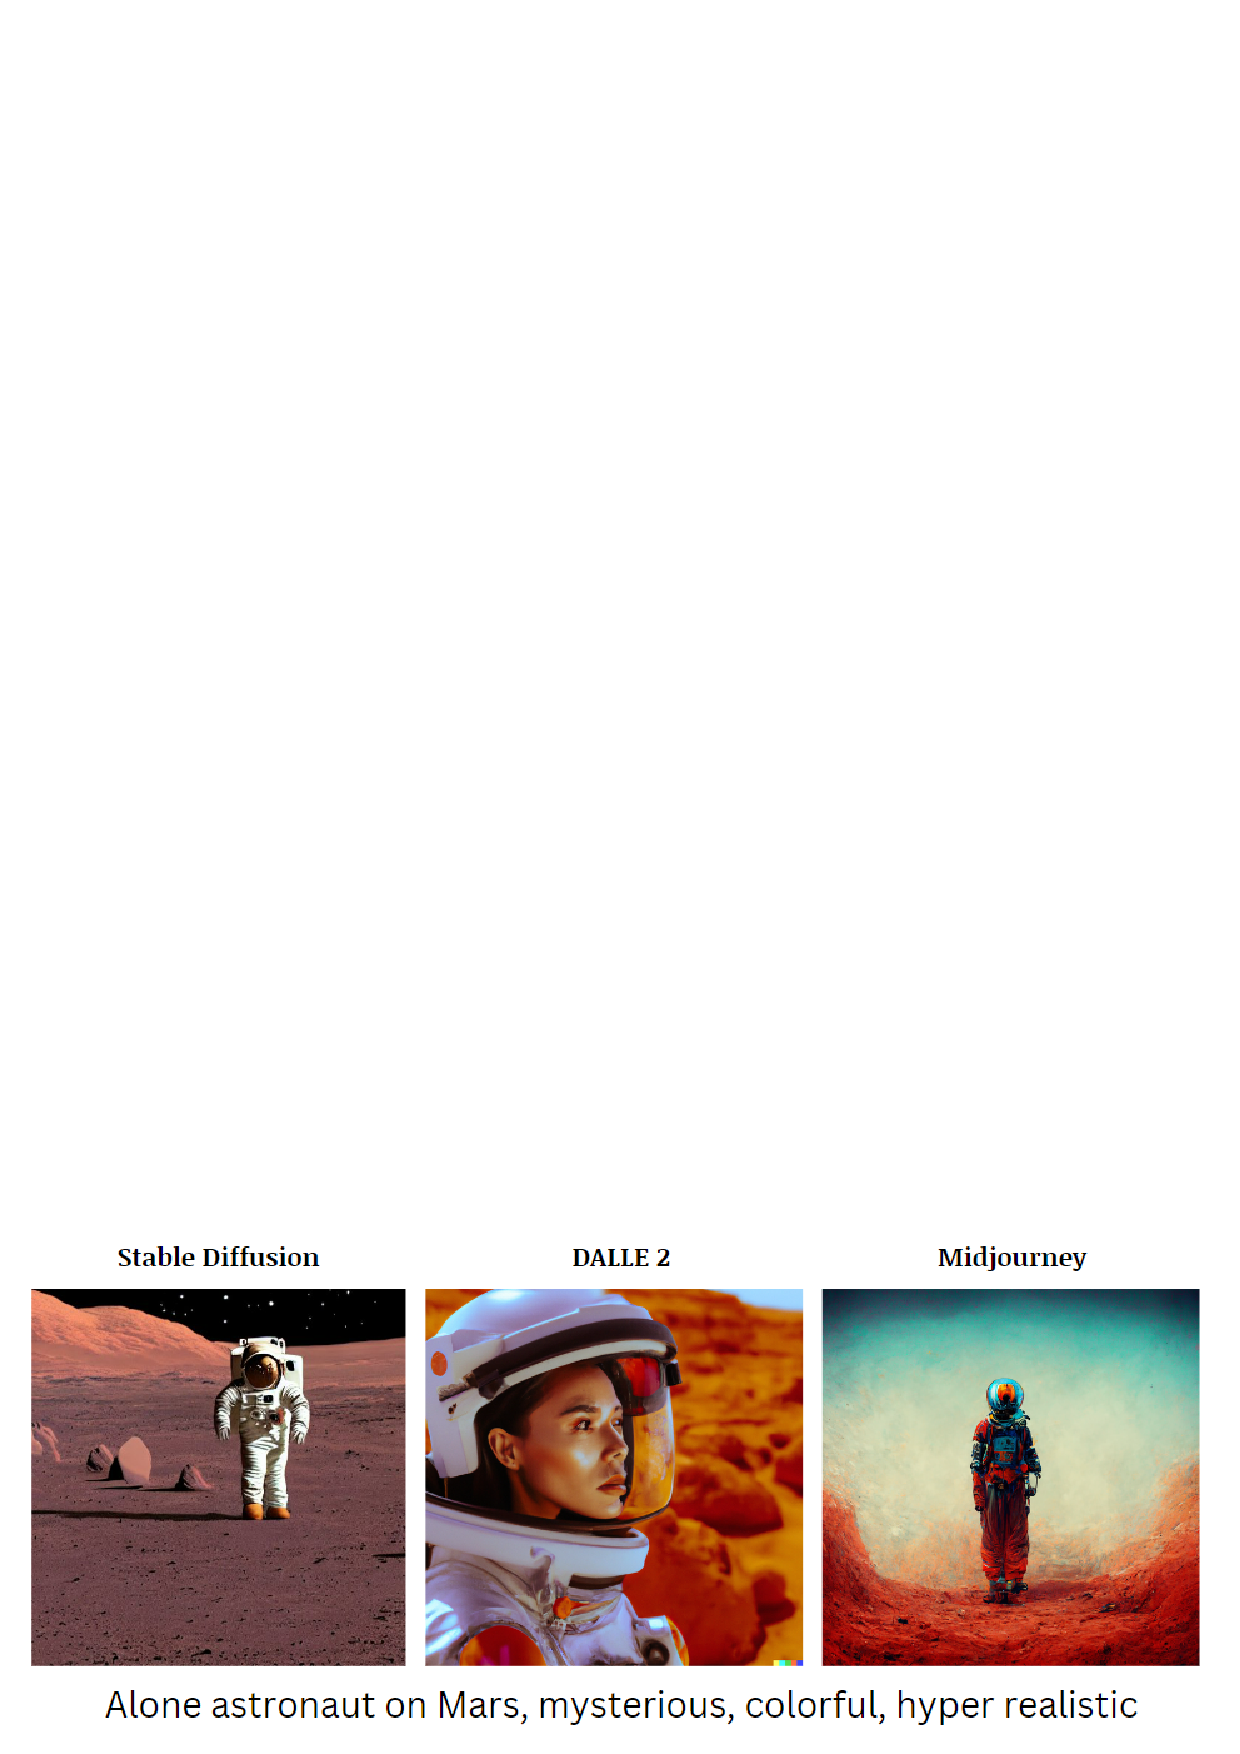
\includegraphics[width=0.8\textwidth]{astronaut.png}
\caption{Poređenje ova tri AI generatora}
\label{fig: Astronaut}
\end{figure}
 
\pagebreak

\section{Etički problemi sa veštačko inteligentnim generatorima slika}

AI generatori slika mogu doprineti diskriminaciji tako što oponašaju štetne stereotipe koje je AI prikupio u kolekcijama podataka, koji sami imaju predrasude iz svakodnevnog života.

U svom članku Rune Klingenberg Hansen nudi sledeća rešenja \cite{kljuc1}. Problem se može korigovati zabranjivanjem određenih reči ili nasumičnim dodavanjem prefiksa kao što su: žena/muškarac/trans, crna/žuta/braon osoba, kvir\footnote{kvir (engl. queer) - naziv za celokupnu homoseksualnu, biseksualnu, transrodnu i interseksualnu zajednicu kao i heteroseksualne osobe koje sebe vide ili žive svoj život van heteropatrijarhalnih normi.} itd.). Ali nekada automatsko dodavanje dodatnih reči može negativno uticati umesto da reši problem. Npr. dodavanje reči žena za neke termine koji se koriste za osobe svih polova ili dodavanje reči crnac kada se spominju bande/kartele.

Još jedan problem je mogućnost veštačke inteligencije da generiše lažne informacije. To je upravo razlog zašto DALL-E \cite{dalle} ne dozvoljava generisanje slika sa poznatim osobama \cite{poznate}, ali lažne informacije ne utiču samo na poznate ljude. Npr. ljudi se mogu svetiti svojim bivšim partnerima ili članovima svoje porodice.

Ali možda najstrašnije stvar jeste da ova tehnologija može u potpunosti uništiti naše poverenje u slike kao verodostojan dokaz. Zbog straha da su slike lažne, jer generator slika nam omogućava da kreiramo fotorealistične slike. Opasnost od ovog scenarija se može umanjiti korišćenjem tehnologija koje imaju sposobnost detektovanja lažnih slika. Takođe mogli bismo zahtevati da veštački generisane slike imaju neku oznaku, pogotovo kada su u pitanju fotorealistične slike.



\subsection{Problem autorskih prava}

Svi mi svakodnevno koristimo slike za razmenjivanje ideja i vizuelna reprezentacija sadržaja je sada više nego ikada dostupna svima nama. Pored lične upotrebe, slike su u savremenom kapitalističkom društvo postale sredstvo promovisanja usluga i proizvoda (naslovnice knjiga, bilbordi itd.). Generatori slika svima nama dozvoljavaju da kreiramo potpuno nove slike i da ih koristimo u komercijalne svrhe, ali onda se javlja pitanje ko polaže autorska prava nad tim generisanim slikama. Da li osoba koja je okucala tekst i pritisnula dugme za generisanje, da nije algoritam koji je izgenerisao sliku ili pak kompanija koja je kreirala algoritam?

Takođe, generatori slike imaju mogućnost da oponašaju umetnički stil mnogih poznatih umetnika. S jednim klikom korisnik može da izgeneriše hiljade slika u stilu Leonarda Da Vinčija. Da li je u tom slušaju korisnik plagirao životno delo slikara? Generator slika ne samo da uzima inspiraciju iz jedne slike umetnika, već kreira slike na osnovu njegovog celokupnog životnog dela.

Na prvu loptu ovo nam zvuči kao očigledan plagijat, ali moramo sagledati širu sliku. Kao što ljudskog biće dobija ispiraciju iz svega što ga okružuje, tako i veštačka inteligencija dobija ispiraciju iz kolekcija podataka koje analizira. U apstraktnom smislu, način na koji čovek i veštačka inteligencija kreiraju slike je dosta sličan. Oboje imaju neku početnu ideju koja proizašla iz informacija koje su dobili na njima prirodan način. Čovek ih dobija preko svojih čula, dok veštačka inteligencija ih, trenutno, dobija u binarnom zapisu na nekom medijumu za skladištenje podataka. Polazeći iz ideje, oboje biraju korake koji ih vode prema tome da završnim proizvod bude njihova lična kreacija. Jedina razlika između čoveka i veštačke inteligencije je činjenica da je veštačka inteligencija mnogo brža i efikasnija u tom procesu. Može se reći da je veštačka inteligencija umnogome sposobnija od čoveka. 

Ukoliko bismo živeli u svetu gde je čovek podjednako inteligentan kao veštačka inteligencija ne bi nam bilo ni čudno ni pogrešno da čovek može da kreira s tolikom preciznošću i brzinom. To što je veštačka inteligencija trenutno samo jedno polje na veb stranici ne treba da nas zavara da će veštačka inteligencija jednog dana, vrlo verovatno, sama stvarati i evoluirati.

Generatori slika stvarno kreiraju problem celokupnoj kreativnoj industriji, ali treba na veštačku inteligenciju posmatrati kao na još jednu alatku koju umetnik može da koristi. Možda upravo uz pomoć veštačke inteligencija umetnost može postani brža, dostupnija i otvorenija \cite{fear}.

\pagebreak

\section{Zaključak}

Dakle, znamo šta je veštačka inteligencija, kako se ona može upotrebiti(ali i zloupotrebiti) za generisanje slika, kako radi, kao i par naših omiljenih primera. Naravno, i dalje postoji mnoga ograničenja, ali i mogućnosti za napredak u oblasti AI-a. Jedna od tih oblasti je generisanje videa iz unetog teksta na čemu radi poznata kompanija Meta\footnote{Meta, nekada Facebook, jedna je od vodećih svetskih biznis magnata u oblasti razvoja veštačke inteligencije i tehnologije.}. 

Oduprećemo se želji da vodimo debatu o tome kako će sve ovo uticati na kreativnu industriju. Međutim, istorija nam sugeriše da pojava novih alata ima tendenciju da proširi definiciju umetnosti. Dakle, \textit{"umetnost nije mrtva, samo je mašinski generisana"}\cite{clanaknov}.

\pagebreak
\begin{thebibliography}{10}

\bibitem{kljucJedan} Schank, R. C. (1987). What Is AI, Anyway?. AI Magazine, 8(4), 59. https://doi.org/10.1609/aimag.v8i4.623  
\bibitem{kljucDva} Dostupno na adresi\begin{verbatim} https://www.cse.unsw.edu.au/~cs9417ml/RL1/introduction.html \end{verbatim}  
\bibitem{kljucTri} Dostupno na adresi\begin{verbatim} https://www.youtube.com/watch?v=yTAMrHVG1ew&t=53s/ \end{verbatim} 

\bibitem{gan1} Stanislav Frolov, Tobias Hinz, Federico Raue, Jörn Hees, Andreas Dengel, Adversarial text-to-image synthesis: A review. Dostupno na adresi https://www.sciencedirect.com/science/article/pii/S0893608021002823
\bibitem{gan2} Scott Reed, Zeynep Akata, Xinchen Yan, Lajanugen Logeswaran, Bernt Schiele, Honglak Lee, Generative Adversarial Text to Image Synthesis. Dostupno na adresi http://proceedings.mlr.press/v48/reed16.pdf/

\bibitem{ganvideo} Computerphile, Generative Adversarial Networks (GANs) - Computerphile. Dostupno na adresi https://www.youtube.com/watch?v=Sw9r8CL98N0/

\bibitem{gen1} Computephile, How AI Image Generators Work (Stable Diffusion / Dall-E) - Computerphile. Dostupno na adresi https://www.youtube.com/watch?v=1CIpzeNxIhU/

\bibitem{openai_dali} Aditya Ramesh, Prafulla Dhariwal, Alex Nichol, Casey Chu, Mark Chen, Hierarchical Text-Conditional
Image Generation with CLIP Latents. Dostupno na adresi https://cdn.openai.com/papers/dall-e-2.pdf/

\bibitem{openai_glide} Alex Nichol, Prafulla Dhariwal, Aditya Ramesh, Pranav Shyam, Pamela Mishkin, Bob McGrew, Ilya Sutskever, Mark Chen, GLIDE: Towards Photorealistic Image Generation and Editing with Text-Guided Diffusion Models. Dostupno na adresi https://arxiv.org/abs/2112.10741/

\bibitem{clip} OpenAI, CLIP: Connecting
Text and Images. Dostoupno na adresi https://openai.com/blog/clip/

\bibitem{asembli} AssemblyAI, How does DALL-E 2 actually work? Dostupno na adresi\begin{verbatim} https://www.youtube.com/watch?v=F1X4fHzF4mQ&t=359s/

\end{verbatim}

\bibitem{difvideo} AssemblyAI, Diffusion models explained in 4-difficulty levels. Dostupno na adresi\begin{verbatim} https://www.youtube.com/watch?v=yTAMrHVG1ew&t=53s/
\end{verbatim}

\bibitem{Prompt}Knjiga je besplatna i dostupna na adresi:\begin{verbatim}https://dallery.gallery/the-dalle-2-prompt-book/\end{verbatim}

\bibitem{kljuc1} Rune Klingenberg Hansen, AI Image Generator: This Is Someone Thinking About Data Ethics. Dostupno na adresi https://dataethics.eu/ai-image-generator-this-is-someone-thinking-about-data-ethics/

\bibitem{dalle} DALL-E 2. Dodatne informacije dostupne na adresi https://openai.com/dall-e-2/

\bibitem{poznate} DALL-E 2 Content policy. Dostupno na adresi https://labs.openai.com/policies/content-policy

\bibitem{fear} Paul Ford, Dear Artists: Do Not Fear AI Image Generators. Dostupno na adresi https://www.wired.com/story/artists-do-not-fear-ai-image-generators/

\bibitem{clanaknov} Guido Appenzeller, Matt Bornstein, Martin Casado, Yoko Li, \textit{Art isn't dead, it's just machine-generated}

\end{thebibliography}

\end{document}
